% ------------------------------------------------------------------
\renewcommand{\thisunit}{MATH327 Unit 10}
\renewcommand{\moddate}{Last modified 10 May 2022}
\setcounter{section}{10}
\setcounter{subsection}{0}
\phantomsection
\addcontentsline{toc}{section}{Unit 10: Synthesis and broader applications}
\section*{Unit 10: Synthesis and broader applications} % TODO: Synthesizing interacting systems with numerical techniques used for computer project...
\subsection{\label{sec:MonteCarlo}Monte Carlo importance sampling}
Although we were able to derive some exact results for the Ising model in one and two dimensions, it's worth recalling that for $3 \leq d < \infty$ no exact solution is known even for this simple system.
In general, interacting statistical systems are not exactly solvable.
In order to explore their broad applications throughout the mathematical sciences and beyond, we therefore need to analyze them either through systematic approximation schemes (such as \emph{perturbation theory}) or by numerical computations.
Numerical methods have become increasingly important over the past fifty years, and in this section we'll outline the general methods they employ.

Our goal is to compute expectation values of interest, which are formally defined by sums over all micro-states.
Considering the canonical ensemble for simplicity,
\begin{equation*}
  \vev{\cO} = \sum_{i = 1}^M \cO_i \; p_i = \frac{1}{Z} \sum_{i = 1}^M \cO_i \; e^{-\be E_i} = \frac{\sum_{i = 1}^M \cO_i \; e^{-\be E_i}}{\sum_{i = 1}^M e^{-\be E_i}}.
\end{equation*}
We already saw, at the end of \secref{sec:Ising}, that enormous computational resources would be required to carry out such sums over micro-states.
Even for tiny Ising systems with $N \sim 1000$ spins, the largest existing or foreseeable supercomputers would have to run for far longer than the age of the universe in order to evaluate the roughly $2^{1000} \sim 10^{300}$ terms in the partition function.
To quantify `tiny', consider that $N \sim 1000$ would correspond to a $10\times 10\times 10$ lattice in three dimensions or a $6\times 6\times 6\times 6$ lattice in four dimensions, both very far from the $N \to \infty$ thermodynamic limit of interest for phase transitions.

And yet, at the end of \secref{sec:mean_field} we were able to quote numerical results for the Ising model critical temperature for $3 \leq d \leq 7$, along with a $d = 3$ critical exponent.
These results are obtainable because practical numerical computations do not perform a `brute-force' evaluation of every single micro-state.
Instead, they proceed by (pseudo-)randomly \textbf{sampling} a very small subset of those micro-states, and using this subset to compute results for the average energy, magnetization, and other thermodynamic quantities.
So long as this sampling is done appropriately, the law of large numbers allows us to treat these averages as controlled approximations to the true ensemble expectation values.

As we saw in the computer project, such numerical calculations employ pseudo-random numbers rather than complete randomness, which allows them to be reproducible up to very high precision by different people using different computers.
Due to the role of randomness, these numerical approaches have become known as \textbf{Monte Carlo} methods, based on a whimsical reference to the famous gambling centre in Monaco.
Monte Carlo methods are crucial in statistical physics, and related disciplines, because they are very broadly applicable to interacting systems that no longer benefit from dramatic simplifications through factorization.

We can gain some intuition about how Monte Carlo methods work by using such pseudo-random sampling to numerically evaluate a simple integral.
The idea is that the integral can be numerically approximated by evaluating its integrand at randomly sampled points in the integration domain, and normalizing by the number of samples.
An amusing example is to compute
\begin{align*}
  \pi & = \int_{-1}^1 dx \int_{-1}^1 dy \ H\!\left(1 - \left\{x^2 + y^2\right\}\right) \qquad &
  H(r) & = \left\{\begin{array}{l}1 \qquad \mbox{for } \ r \geq 0 \\
                                  0 \qquad \mbox{for } \ r < 0\end{array}\right. ,
\end{align*}
where the Heaviside step function $H(r)$ picks out a disk with radius $R = 1$ in a square integration domain with area $4$, as shown below.
Since the integrand is either $0$ or $1$ for each randomly sampled point in that domain, simply counting the fraction of the $S$ samples that lie in the disk provides a numerical determination of $\pi$, with a \textit{statistical uncertainty} that vanishes $\propto 1 / \sqrt{S}$.
In just a few minutes, \href{https://github.com/daschaich/MATH327_2022/blob/master/lecture_notes/unit10_pi.py}{this Python code} predicts $\pi = 3.14152 \pm 0.00023$ purely from sampling pseudo-random numbers.

\begin{center}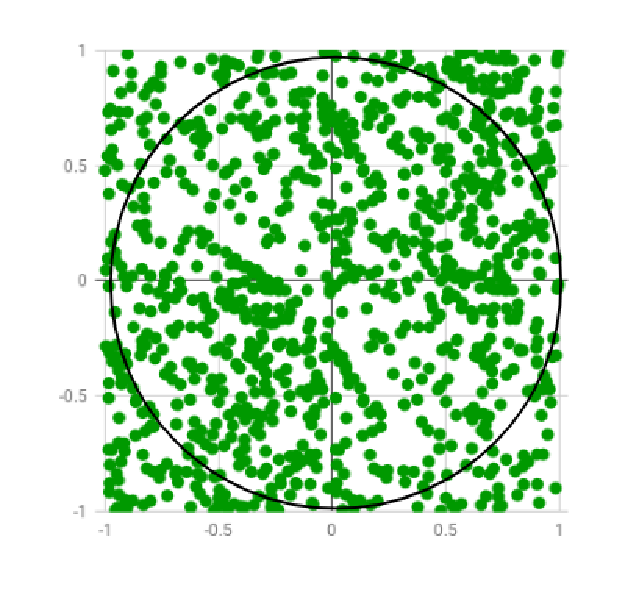
\includegraphics[width=0.6\textwidth]{figs/unit10_pi.pdf}\end{center}

Of course, numerically computing $\pi$ can be done far more efficiently with other, more specialized, techniques.
Monte Carlo integration is most useful when we need to consider very high-dimensional integrals --- such as partition functions of interacting statistical systems, interpreted as $N$-dimensional integrals over the system's $N$ degrees of freedom.
To illustrate the scale of computations that can currently be carried out, ongoing theoretical physics research here in Liverpool routinely uses Monte Carlo methods to numerically evaluate roughly billion-dimensional integrals.

At this point, you might be concerned that such sampling can account for only an extremely small fraction of the possible micro-states for the systems under consideration, suggesting a risk of inaccurate results from unrepresentative sampling.
This is a new manifestation of the obstacle we encountered when considering brute-force computations above.
If the brute-force evaluation of every single micro-state takes far longer than the age of the universe, then the fraction we could sample in a reasonable amount of time (say, a day) is almost vanishingly small.

As a concrete example, if we generously suppose our computer only needs a few nanoseconds to sample a micro-state of a tiny $N \sim 1000$ Ising system, over the course of a day it would sample roughly ten trillion ($10^{13}$) spin configurations --- only about one part in $10^{287}$ of the total $2^N \sim 10^{300}$ micro-states.
To make the situation even worse, as $N$ increases the number of possible Ising model micro-states grows \textit{exponentially} quickly, $\sim$$2^N$, in addition to the more modest growth in the amount of computing required to sample each micro-state.
For illustration, 2015 research \href{https://arxiv.org/abs/1502.07613}{arXiv:1502.07613} numerically predicting $T_c$ for the Ising model in $d = 5$, $6$ and $7$ dimensions includes calculations up to $N = 64^5 \approx 10^9$.
Out of the roughly $2^{10^9} \sim 10^{323{,}000{,}000}$ micro-states for this systems, only $\sim$$10^4$ could be sampled in a reasonable amount of time.
How much trust should we place in results from such numerical work?

Thinking back to our consideration of the ordered and disordered phases of the Ising model in \secref{sec:Ising_phases}, we could make a case that everything may work out in the high-temperature disordered phase.
In the infinite-temperature limit, all the micro-states become equally probable, and observable expectation values are determined by the degeneracies of the different energy levels.
Random sampling is more likely to account for the dominant energy levels with large degeneracies, making it plausible that reasonable results could be obtained by averaging even over such a tiny fraction of the total number of micro-states.

In the low-temperature ordered phase, however, the opposite occurs.
As the temperature decreases, the large-scale behaviour of the system in this phase is dominated by a very small number of micro-states.
For sufficiently low temperatures, observable expectation values are effectively determined by the two degenerate minimum-energy micro-states with all spins aligned either up or down.
Only exponentially suppressed corrections would then be introduced by higher-energy excited states.
As there is essentially no chance of randomly sampling either of those two minimum-energy micro-states, the random sampling approach described above seems doomed to fail.

A key breakthrough that made numerical results truly reliable was the invention of stochastic procedures to sample any micro-state $\om_i$ with a probability proportional to its Boltzmann factor, $p_i \propto e^{-\be E_i}$.
Such automated procedures are known as \textit{algorithms} (a term that evolved from the name of \href{https://en.wikipedia.org/wiki/Muhammad_ibn_Musa_al-Khwarizmi}{Muhammad ibn Musa al-Khwarizmi}), and the overall approach is called \textbf{importance sampling}, since it preferentially samples the important micro-states that make the most significant contributions to the partition function and derived quantities. % TODO: Persian mathematician active in the early 9th century...
Assuming we have such an algorithm, applying it to the $\be \to \infty$ low-temperature phase considered above would produce an exponentially enhanced probability of sampling low-energy micro-states, as desired.
As $\be \to 0$ in the high-temperature phase, there would be little change compared to the more straightforward pseudo-random sampling considered above, since all micro-states would become equally probable.

The challenge is to design importance sampling algorithms in the first place.
In particular, these algorithms can't rely on knowing the full set of micro-state energies $E_i$, and the corresponding probabilities $p_i$, since enumerating these data would be equivalent to brute-force computation of the full partition function.
In essence, the algorithm has to exploit its stochastic aspect --- its use of pseudo-random numbers --- to guide it to important, high-probability micro-states.
And this guiding needs to be done without introducing any other bias that might cause distorted results to be obtained from averaging over the tiny fraction of micro-states that can be sampled in a reasonable amount of time.

A \href{https://en.wikipedia.org/wiki/Equation_of_State_Calculations_by_Fast_Computing_Machines}{famous solution} to this challenge was developed in 1953 by \href{https://en.wikipedia.org/wiki/Nicholas_Metropolis}{Nick Metropolis}, \href{https://en.wikipedia.org/wiki/Arianna_W._Rosenbluth}{Arianna Rosenbluth}, \href{https://en.wikipedia.org/wiki/Marshall_Rosenbluth}{Marshall Rosenbluth}, \href{https://en.wikipedia.org/wiki/Augusta_H._Teller}{Mici Teller} and \href{https://en.wikipedia.org/wiki/Edward_Teller}{Edward Teller}.
I will call this solution the Metropolis--Rosenbluth--Teller algorithm, or the MRT algorithm for short.\footnote{In an infamous misfiring of alphabetical ordering, this remains widely known as the ``Metropolis algorithm'' even though Metropolis's role was providing specialized computing equipment rather than creating the algorithm itself.  In addition, the key contributions of Arianna Rosenbluth and Mici Teller were widely under-appreciated for many years.}
It relies on the concept of Markov chains that we briefly discussed when considering random walks all the way back in \secref{sec:diffusion}.
To reiterate the key concept, a Markov chain is a process in which the next micro-state to be sampled is pseudo-randomly chosen based on the micro-state currently under consideration, with no `memory' of any other micro-states that may previously have been sampled.

We can use the Ising model to illustrate how the MRT algorithm employs Markov chains to sample micro-states proportionally to their importance.
Any spin configuration can serve equally well as the initial micro-state at the start of the chain.
Starting from this initial configuration, we pseudo-randomly select one spin, $s_j$, and compute $\De E_j$, the change in the system's energy that would be caused by flipping $s_j \to -s_j$.
We then update the spin configuration by `accepting' this spin flip with probability
\begin{equation}
  \label{eq:MRTprob}
  P_{\text{accept}} = \mbox{min}\left\{1, e^{-\be \De E_j}\right\},
\end{equation}
which defines the next micro-state in the Markov chain.
Importantly, this new micro-state may be identical to the previous micro-state --- this occurs with probability $P_{\text{reject}} = 1 - P_{\text{accept}}$.
The final step of the algorithm is to repeat this single-spin update procedure as many times as our computers can handle.

We can appreciate why micro-states may need to be repeated in the Markov chain by considering what should happen if we were to sample the ground state at low temperatures.
In this regime, the ground state should dominate, so the algorithm should sample it repeatedly, proportionally to its probability.

Digging into \eq{eq:MRTprob}, we can see that any spin flip that lowers the energy will always be accepted, since $\De E < 0 \implies e^{-\be \De E} > 1$.
The MRT algorithm is therefore free to approach the minimum-energy ground state of the system.
If it is in the ground state, then any spin flip will increase the energy, $\De E > 0$, and will only be accepted with an exponentially suppressed probability $e^{-\be \De E} \to 0$ as $T = 1 / \be \to 0$, as desired.
More generally, if we consider two micro-states $\om_A$ and $\om_B$, then the relative probabilities of moving between these two micro-states are
\begin{equation}
  \label{eq:MRTdistribution}
  \frac{P(A \to B)}{P(B \to A)} = \frac{\mbox{min}\left\{1, e^{-\be(E_B - E_A)}\right\}}{\mbox{min}\left\{1, e^{-\be(E_A - E_B)}\right\}} = \frac{e^{-\be(E_B - E_A)}}{1} = \frac{e^{-\be E_B}}{e^{-\be E_A}},
\end{equation}
regardless of whether $E_A \leq E_B$ or $E_B \leq E_A$.

So long as every micro-state can be generated from any other micro-state by making a series of pseudo-random changes to individual degrees of freedom, \eq{eq:MRTdistribution} ensures that the micro-states $\om_i$ will indeed be sampled with probabilities proportional to the Boltzmann factors $e^{-\be E_i}$ that quantify their importance.
The necessary condition that the Markov chain can reach every micro-state (at least in principle) is called \textbf{ergodicity}.
Because the micro-state probabilities $p_i$ are effectively `felt out' through the accept/reject test described above, in non-ergodic situations the algorithm will fail to account for the probabilities of micro-states that can't be reached by the Markov chain.
This can easily lead to incorrect results.

You can read more about the MRT algorithm in Section~8.2 of Dan Schroe-der's \textit{Introduction to Thermal Physics} (the second item in the list of further reading on page~5), which provides a single-page annotated code implementing it for the two-dimensional Ising model. % WARNING: Hyphenating by hand
While the conceptually simple MRT algorithm is the most famous means to carry out Markov-chain Monte Carlo importance sampling, it is far from the only option, and often far from the best.
If time permits, we may discuss some of the challenges that make it advantageous to go beyond the MRT algorithm, in particular the issue of \textbf{auto-correlations}.

For now, suffice it to say that there is an enormous amount of ongoing research developing, optimizing and applying more elaborate Monte Carlo methods to investigate topics throughout the mathematical sciences and beyond.
In \secref{sec:broad} we will briefly look at some of these broader applications.
First, there is another important concept to introduce, called universality, which helps to reveal why interacting statistical systems are so useful to apply to such a diverse range of scientific investigations.
% ------------------------------------------------------------------



% ------------------------------------------------------------------
\subsection{Universality}
In \secref{sec:mean_field} we defined the critical exponent $b$ as the power governing the behaviour of the order parameter $\vev{m} \propto \left(T_c - T\right)^b$ as the temperature $T$ approaches the critical temperature $T_c$ of the second-order phase transition.
In addition to being an important feature characterizing any given phase transition, it was discovered during the twentieth century that precisely the same critical exponents turn out to govern the behaviour of phase transitions that we initially would not have expected to have any connection.
For example, the critical exponent $b \approx 0.32$ for the three-dimensional Ising model magnetization mentioned last week also appears at the phase transition where an interacting (non-ideal) gas transforms into a liquid,
\begin{align*}
  \frac{1}{\rho_{\text{gas}}} - \frac{1}{\rho_{\text{liquid}}} & \propto \left(T_c - T\right)^b &
  b & \approx 0.32,
\end{align*}
where $\rho$ is the density of the atoms, which are equal for the two phases at the transition.\footnote{We're not covering the liquid--gas transition in this module.  If you are curious about it, you can find a discussion in Section~5.1 of David Tong's \href{https://www.damtp.cam.ac.uk/user/tong/statphys.html}{\textit{Lectures on Statistical Physics}} (reference~1 in the list of further reading on page~6).}

This is not simply a numerical coincidence, but an example of an amazing phenomenon is known as \textbf{universality}.
In essence, universality states that the specific details of interacting statistical systems become irrelevant close to critical points at which phase transitions occur.
It doesn't matter whether we are considering a three-dimensional lattice of Ising spins or a liquid such as water---the behaviour of both systems is governed by the same set of critical exponents (known as their \textit{universality class}).

The detailed mathematics underlying universality is well beyond the scope of this module.
Important contributions to its development were made by \href{https://en.wikipedia.org/wiki/Leo_Kadanoff}{Leo Kadanoff} and \href{https://en.wikipedia.org/wiki/Kenneth_G._Wilson}{Ken Wilson}, among many others.
The purpose of this section is just to quickly introduce the concept and emphasize that universality causes the same large-scale behaviour to appear in the vicinity of critical points even for systems that initially may seem completely different.
This independence of the details of the system helps to explain the power of even simple interacting statistical systems such as the Ising model, and their applicability in so many different domains.
% ------------------------------------------------------------------



% ------------------------------------------------------------------
\subsection{\label{sec:broad}Broader applications}
In this section we will continue to provide quick introductions rather than detailed derivations, considering a few ways in which the concepts and tools of statistical physics are applied beyond the mathematical sciences.
The cases considered here are far from exhaustive, and many more examples may become apparent now that we have gained familiarity with the underlying statistical methods and perspectives.

\subsubsection*{Voter models}
Sociology is one domain where the applicability of statistical physics may be unexpected.
Despite (possible) expectations, there is a diverse and active field of ``sociophysics'', which uses the statistical physics concepts and tools that we have been learning about to describe various aspects of social and political behavior.\footnote{For a review, see Serge Galam, \href{https://liverpool.idm.oclc.org/login?url=http://dx.doi.org/10.1007/978-1-4614-2032-3}{\textit{Sociophysics: A Physicist's Modeling of Psycho-political Phenomena}} (2012).}

A particular branch of sociology where connections to statistical physics may be more apparent is the field of opinion formation, where so-called \href{https://en.wikipedia.org/wiki/Voter_model}{voter models} have been widely used since the 1970s, and have proved capable of capturing outcomes of elections.
Voter models are interacting statistical systems not too different from the Ising model, where spin degrees of freedom that we have been working with are interpreted as voters' opinions on a certain topic.
For example, support for a proposal or candidate can be represented as $s_i = +1$, while opposition would be $s_i = -1$.
Just like the interactions in the Ising model encourage spins to align with each other, voter models build in a tendency for voters to align (i.e., agree) with the majority of other voters they interact with.

There are many generalizations that can then be incorporated to better describe the outcome of polls and elections.
A simple extension would be to allow voters to be neutral or indifferent to the question, represented as $s_i = 0$.
Similarly, the strength of a voter's commitment to their opinion can be modelled by extending the range of possible spin values,
\begin{equation*}
  s_i \in \left\{\cdots, -2, -1, 0, +1, +2, \cdots\right\}.
\end{equation*}

Another way to make voter models more realistic is to define them on more flexible \textit{graphs} rather than regular lattices.
The figure below (\href{https://doi.org/10.1073/pnas.1200709109}{source}) illustrates how such a graph can look for a two-state system with $s_i \in \left\{-1, +1\right\}$ coloured red and blue.
As in everyday experience (and inspired by social networks), different voters can have connections with different numbers of other voters, who do not need to be nearest neighbours.
In this particular investigation, network connections between disagreeing voters are probabilistically severed, and transitions are observed between a phase in which one of the opinions becomes the consensus, or all connections are severed between the two groups with differing opinions.

\begin{center}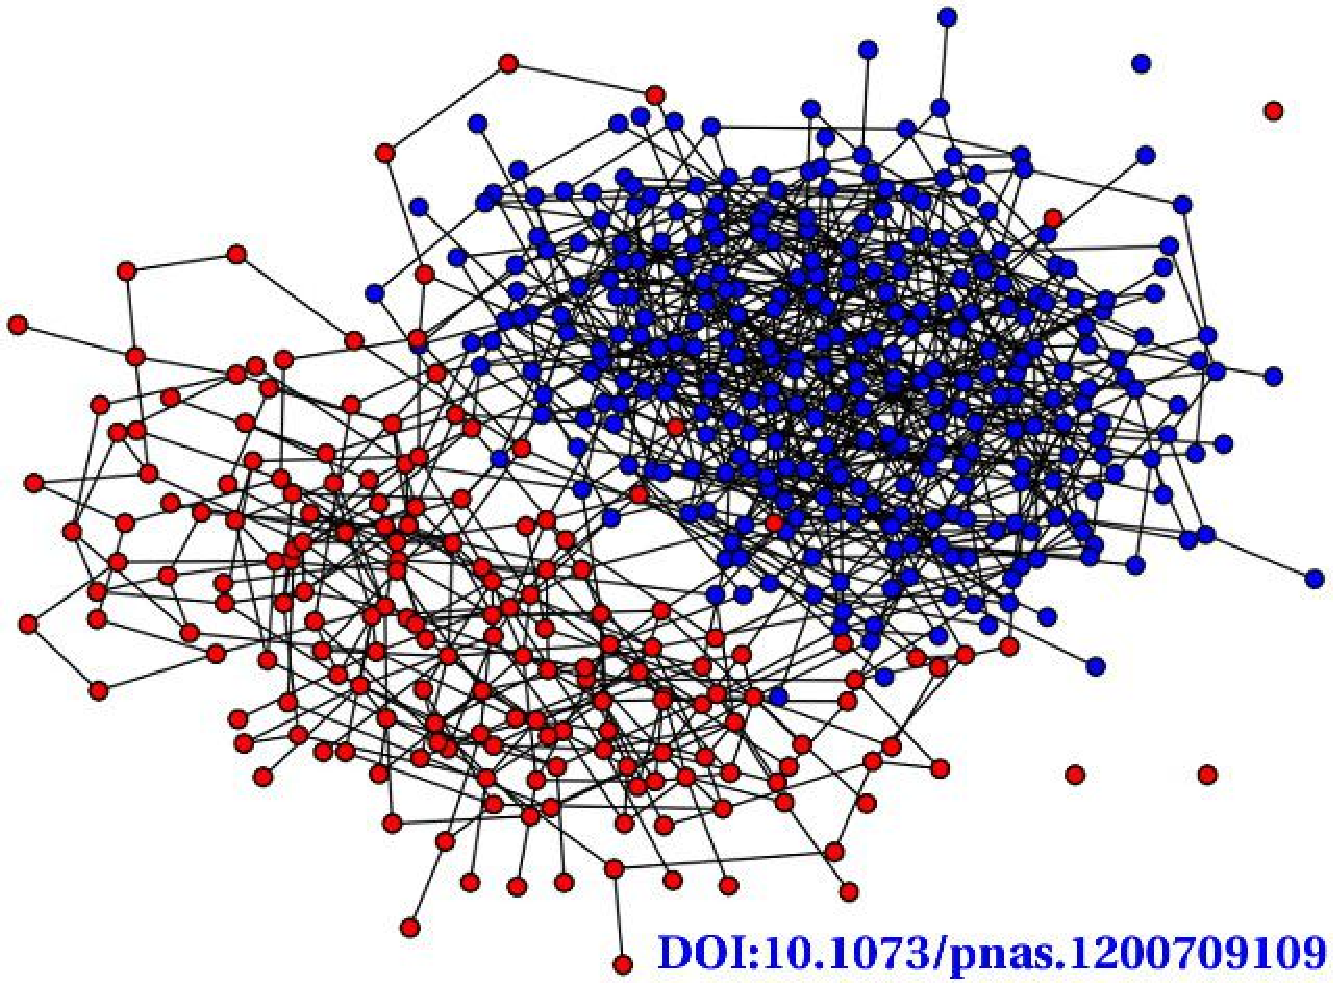
\includegraphics[width=0.7\textwidth]{figs/unit10_voter.pdf}\end{center}

Simpler studies that don't involve severing connections have observed a similar consensus phase occurring once an opinion reaches a critical concentration.
Remarkably, this was found to be described by a second-order phase transition in the universality class of the two-dimensional Ising model.
Another outcome possible in certain voter models is a ``stable non-consensus'' phase, in which the two opinions persist indefinitely, each one held by a `cluster' of aligned voters who interact mainly with each other rather than with voters holding the opposite opinion.
These investigations are described by Alexander Balankin et al., ``\href{https://doi.org/10.1016/j.physleta.2016.12.001}{Ising percolation in a three-state majority vote model}'' (2016).

\subsubsection*{Epidemiology}
A particularly topical application of interacting statistical systems is to model the spread of diseases in populations, something most of us may have seen in the news over the past fifteen months.
As in the case of voter models, the degrees of freedom under consideration are again individuals, whose interactions with each other allow infection to spread to those who are susceptible.
A Monte Carlo calculation of the sort described in \secref{sec:MonteCarlo} can then be used to model how many people may be infected as time passes, guided by data on typical movement and contacts.

The figure below comes from \href{https://www.washingtonpost.com/graphics/2020/world/corona-simulator/}{an over-simplified simulation} provided by the \textit{Washington Post} to illustrate these concepts.
Here individuals are modeled simply as a gas of interacting particles in two dimensions, and various ways of restricting their motion are used to explore the likely effects of measures such as quarantines and social distancing.
By coincidence, the scale of this simulation, which considers a population of just $200$ people, is comparable to the first importance sampling Monte Carlo calculation carried out in 1953, as a first application of the MRT algorithm, which computed the pressure (i.e., equation of state) for $224$ interacting particles in a two-dimensional `volume'.
At the time, this required several days of computing time on a state-of-the-art machine; now these sorts of calculations are easily done on a smartphone.

\begin{center}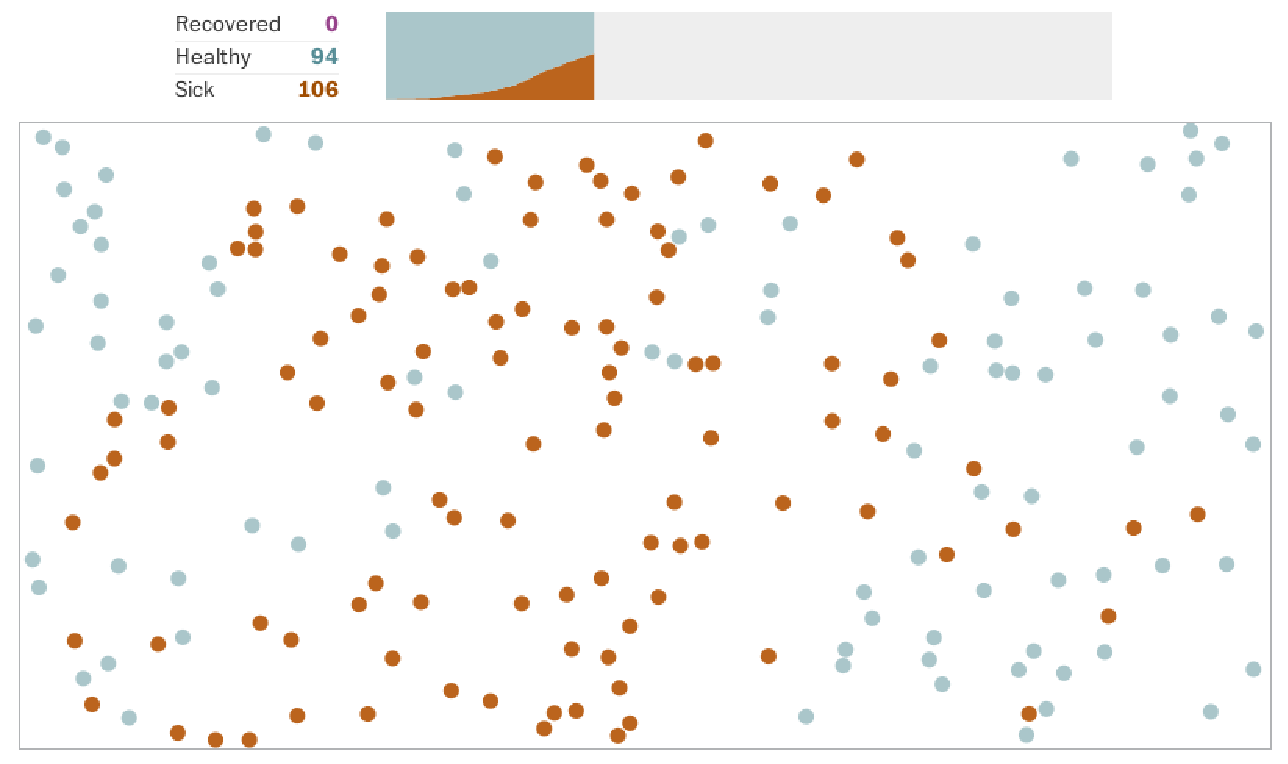
\includegraphics[width=0.8\textwidth]{figs/unit10_epidemic.pdf}\end{center}

Larger-scale and more realistic versions of these epidemiological simulations provide important input into government deliberations regarding what restrictions (such as lockdowns) would be most beneficial to reduce the spread of disease, and how long such restrictions may need to be maintained.
Rather than investigating a phase transition, the goal is to quantify likely effects of restrictions (or of the absence of restrictions).
As described in \secref{sec:LLN}, the numerical experiments are therefore repeated many times with different sequences of pseudo-random numbers.
This produces an ensemble of possibilities from which the likely outcomes of various interventions can be inferred.

\subsubsection*{Flocking}
Let's conclude our quick glimpses of some broader applications of statistical physics by considering another biological example, where interacting statistical systems are used to model the large-scale collective motion of certain groups of animals.
The image below (from Marcus Woo, ``\href{https://www.sciencemag.org/news/2014/07/how-bird-flocks-are-liquid-helium}{How bird flocks are like liquid helium}'', \textit{Science}, 27 July 2014) illustrates the so-called flocking behaviour of large groups of starlings, which fly through the sky in surprisingly tight coordination.
This same sort of behaviour is also seen in schools of fish, swarms of insects, and even crowds of humans.

\begin{center}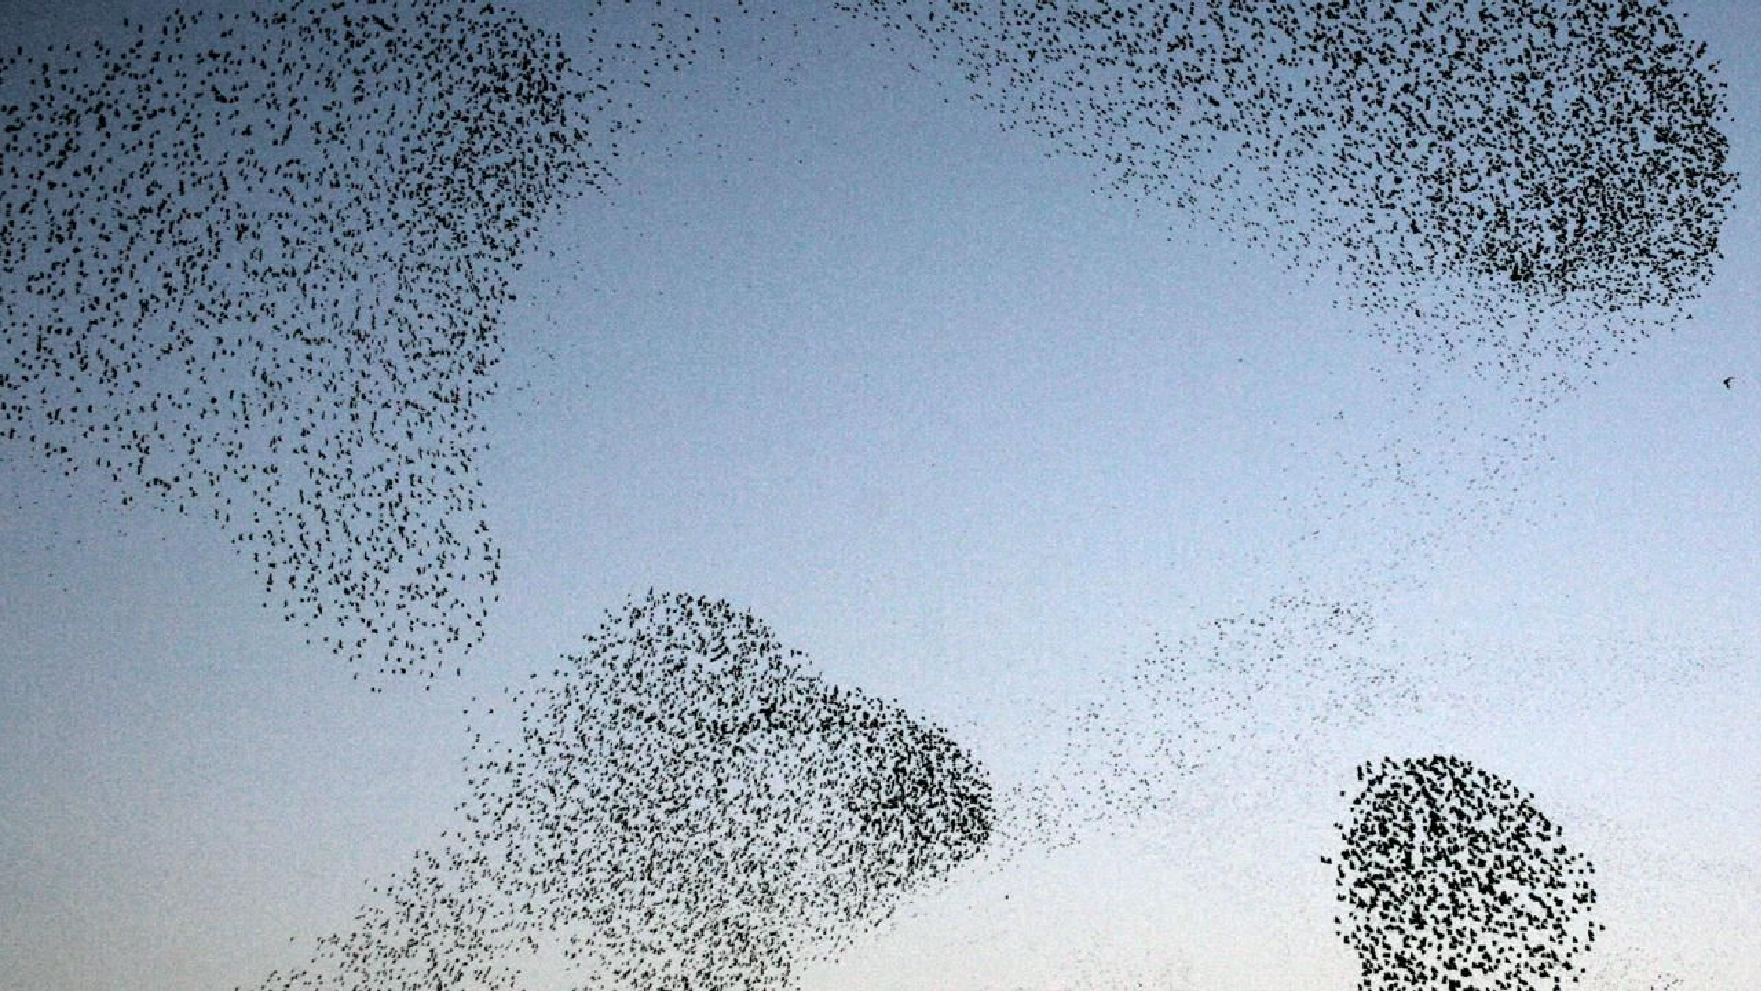
\includegraphics[width=0.8\textwidth]{figs/unit10_flock.pdf}\end{center}

Many models based on interacting statistical systems have been (and continue to be) developed to describe this emergent collective behaviour.
A particularly simple and widely studied \href{https://en.wikipedia.org/wiki/Vicsek_model}{example} was introduced in 1995.
It proposes that each particle (i.e., bird) will interact with others near to it, and this interaction will encourage it to move in the same direction as its neighbours, in much the same way that the nearest-neighbour interactions in the Ising model encourage its spins to align.

This model exhibits a transition between two distinct phases.
When there is a low density of particles, there are relatively few interactions and the particles' motion is disordered, with no formation of flocks or swarms.
At high densities, in contrast, large-scale collective motion appears, based solely on the interactions between the individual particles in the system.
These two regimes turn out to be separated by a first-order phase transition, with a discontinuity (in the thermodynamic limit) in an order parameter related to the average angle of flight.
In addition, as the critical density is approached, flights in the disordered phase exhibit anomalous super-diffusion like that investigated in the computer project.
% ------------------------------------------------------------------



% ------------------------------------------------------------------
\subsection{Wrap-up recap and synthesis}
We have covered a lot of ground in this module, building on foundations from probability theory to develop and apply the core concepts of statistical physics.
In week~1 we defined probability spaces, expectation values and variances, and used these to establish the law of large numbers through which stable large-scale behaviour occurs for stochastic systems involving many degrees of freedom $N \gg 1$.
We also saw how the central limit theorem relates large-$N$ probability distributions to the underlying mean and variance of the elementary degree of freedom, and practiced extracting probabilities from such distributions.
The law of diffusion results from the central limit theorem, and the computer project applied inverse transform sampling to study how anomalous diffusion can arise when the central limit theorem's assumption of finite elementary mean and variance breaks down.

Starting in week~2 we specialized to particular probability spaces known as statistical ensembles, which consist of the micro-states and associated probabilities that a system can possibly adopt through its time evolution.
The laws of physics, such as conservation of energy (the first law of thermodynamics), impose constraints on statistical ensembles.
The micro-canonical ensemble directly implements such constraints, by requiring the system's internal energy and particle number be constant, which implies that the system is completely isolated from the rest of the universe.
This makes both the entropy (\eq{eq:entropy}) and temperature (\eq{eq:temperature}) derived quantities, which we explored via non-interacting spin systems.
In particular, we derived a form of the second law of thermodynamics, which states that the total entropy never decreases as time passes and therefore indicates that maximal entropy corresponds to thermodynamic equilibrium.

Motivated by the impracticality of demanding that a system be completely isolated, in week~3 we turned to the canonical ensemble, which allows systems to exchange energy with a large thermal reservoir that imposes a constant temperature.
The particle number is still fixed, while the entropy, internal energy and heat capacity are now important derived quantities, with the last two related by a fluctuation--dissipation relation.
Maximizing the entropy to consider systems in thermodynamic equilibrium defines the partition function (\eq{eq:canon_part_func}) and Boltzmann distribution (\eq{eq:canon_prob}).
Derived quantities are determined from the partition function, or equivalently the Helmholtz free energy (\eq{eq:helmholtz}).
By analyzing both distinguishable and indistinguishable non-interacting spins, we demonstrated that the intrinsic information content of statistical systems has physically measurable effects.

In week~4 we developed another application of the canonical ensemble by analyzing non-relativistic, classical, ideal (non-interacting) gases.
At the start of this analysis we had to take care to ensure that the partition function was well-defined, by assuming that only discrete momenta are possible in a finite volume $V$, to ensure that the number of micro-states is countable.
Again determining the internal energy (\eq{eq:ideal_energy}) and entropy (\eq{eq:ideal_entropy}) from the resulting partition functions for both distinguishable and indistinguishable gas particles, we computed the mixing entropy that is created by combining gases of distinguishable particles.
Finally we defined the pressure as the adiabatic change in the system's energy upon changing its volume (\eq{eq:pressure}), and derived the ideal gas law (\eq{eq:ideal_gas_law}) as a famous equation of state.

Building on our analyses of ideal gases in the canonical ensemble, in week~5 we considered thermodynamic cycles as systems that perform a repeatable sequence of expansions, compressions and heat transfers in order to act as heat engines or refrigerators.
This required first considering the work done on the system through these processes (\eq{eq:work}), the heat added to or removed from it (\eq{eq:heat_def}), and the first law of thermodynamics expressed in terms of these quantities (\eq{eq:first_law}).
After introducing $PV$~diagrams as a convenient way to visualize thermodynamic cycles and the individual processes that comprise them, we analyzed the Carnot heat engine and computed how much work it can do by transferring heat from a hot thermal reservoir to a cold reservoir.
This combination of work and heat defines the efficiency (\eq{eq:efficiency}), and we computed that the Carnot heat engine achieves the maximum possible efficiency allowed by the second law of thermodynamics.

The logical next step, after allowing the energy to fluctuate with a constant temperature, is also allowing the system to exchange particles with a large particle reservoir.
This leads to the grand-canonical ensemble that we developed in week~6, beginning by defining the chemical potential (\eq{eq:chem_pot}) as the new quantity (in addition to the temperature) that the particle reservoir keeps constant.
Carrying out another round of entropy maximization defined the grand-canonical partition function (\eq{eq:grand_part_func}) and the corresponding grand-canonical potential (\eq{eq:grand_pot}) that determine the derived quantities that now include the particle number in addition to the energy and entropy.
We were also able to derive a generalized thermodynamic identity (\eq{eq:thermo_ident}) that relates the chemical potential to the change in energy upon adiabatically adding a particle to the system.

Our main applications of the grand-canonical ensemble were to analyze gases based on the quantum statistics that we introduced (as an ansatz) in week~7.
After demonstrating how the classical (non-quantum) approach we took when first considering ideal gases breaks down when there is a non-negligible probability for multiple identical particles to occupy the same energy level, we got around this problem by organizing the micro-states in terms of the possible occupation numbers of the energy levels.
These possible occupation numbers distinguish between the two types of particles that appear in nature: bosons that can have any non-negative occupation numbers $n_{\ell} \in \Nbb_0$, and fermions that obey the Pauli exclusion principle and can have only $n_{\ell} \in \left\{0, 1\right\}$.
We derived the respective Bose--Einstein and Fermi--Dirac statistics for these two types of quantum particles, and checked that both approach classical (Maxwell--Boltzmann) statistics in the limit of high temperature with large negative chemical potential $-\mu \gg T$.

We carried out a more thorough application of the grand-canonical ensemble to quantum gases of bosons in week~8, focusing on ideal (non-interacting) gases of ultra-relativistic photons with energies defined in terms of frequencies (\eq{eq:photon_omega}).
Based on the grand-canonical potential, we derived the Planck spectrum (\eq{eq:Planck_omega}) governing the frequency dependence of the energy density for photon gases, and found how it solves the ultraviolet catastrophe of the classical Rayleigh--Jeans spectrum.
We also saw how the Planck spectrum provides an excellent mathematical model for both stars (some of the hottest places in the universe) as well as the cosmic microwave background that fills frigid inter-galactic space and provides strong evidence for the existence of dark matter.
We finally derived the radiation pressure of photon gases, and the corresponding equation of state, which has the same form as the ideal gas law, just with a different numerical factor.

In week~9 we carried out a similar application of the grand-canonical ensemble to quantum gases of non-interacting fermions, focusing mainly on non-relativistic particles and considering the low-temperature regime where quantum Fermi--Dirac statistics differs the most from the classical case.
Again based on the grand-canonical potential, we derived the Fermi function $F(E)$ and saw how it becomes a step function at low temperatures.
This corresponds to all the low-lying energy levels being filled by the single fermion that can occupy each of them by the Pauli exclusion principle, up to the Fermi energy that (at zero temperature) is simply the chemical potential (\eq{eq:Fermi_energy}).
The resulting internal energy (\eq{eq:fermi_E_N}) and pressure (\eq{eq:degen_pressure}) remain positive even as the temperature approaches absolute zero.
This non-zero degeneracy pressure helps to explain the regularity of type-Ia supernovas, which play a key role in establishing the existence of so-called dark energy.

The last major topic of the module was to explore effects of interactions in weeks~10 and 11.
Statistical systems in which the constituent degrees of freedom can interact with each other exhibit a broader array of phenomena, such as phase transitions.
At the same time, they become enormously more difficult to analyze, because their partition functions and derived quantities no longer factorize into independent single-particle contributions.
We focused on the famous Ising model, which is simple to write down as a system of spins interacting with their nearest neighbours on a $d$-dimensional simple cubic lattice, but extremely difficult to solve exactly in two or more dimensions.
We discussed how to analyze the Ising model through the mean-field approximation (last week) and by using numerical Monte Carlo importance sampling algorithms (\secref{sec:MonteCarlo}).
For $d \geq 2$, the Ising model exhibits a second-order phase transition between its high-temperature disordered phase and its low-temperature ordered phase.
The critical exponents characterizing these transitions also arise in many other contexts, a phenomenon known as universality, which helps to explain the broad applicability and far-reaching power of statistical physics, including the examples briefly considered in \secref{sec:broad}.

In summary, we have learned foundations including statistical ensembles, entropy, and the laws of thermodynamics.
We have studied applications including diffusion, ideal gases, thermodynamic cycles, and phase transitions.
And we have previewed advanced topics including numerical methods and universality.
All together, our new knowledge of statistical physics enables us to observe and appreciate many further applications of these concepts and tools across the mathematical sciences and beyond.
% ------------------------------------------------------------------
